\section{Supporting result: the discounted objective in one dimension}
\label{app:braking}
% src: docs/findings/braking-gamma.md (table, figure, reading); src/apexzero/learn/braking.py
%      (problem definition, Pontryagin switch, value iteration); scripts/braking_study.py
%      (grid 801 x 361, 41 actions, gammas). docs/STATUS.md (K3 row) for the
%      "one control step" reading.

The answer key solves the agent's discounted objective rather than a minimum-time problem
(\cref{sec:answer-why}). A one-dimensional braking problem, where both optima can be
computed exactly, shows when the distinction matters.

\paragraph{Problem} A point mass on the default car's speed-dependent acceleration envelope
(the one the quasi-steady-state oracle uses) enters a straight at 288\,km/h and must pass
a corner at $s_c = 400$\,m no faster than 90\,km/h; arriving faster is a crash.
% src: src/apexzero/learn/braking.py (BrakingProblem: s_c 400, v_c 25 m/s, v0 80 m/s)
\emph{Minimum time.} The Hamiltonian is linear in the acceleration, so Pontryagin's
principle gives a bang-bang solution: full throttle, then full braking from the point where
the acceleration curve meets the braking curve that ends at $(s_c, v_c)$. That switch
point is at 320.4\,m.
% src: docs/findings/braking-gamma.md (first paragraph)
\emph{Discounted RL.} The agent's objective uses the environment's reward: progress/10\,m
per 50\,ms step, the environment's crash penalty $-(5 + 5(v/50)^2)$ ending the episode, and,
after a safe pass, the discounted progress of 30\,s at full throttle. Value iteration on
an $801 \times 361$ grid in $(s, v)$ with 41 acceleration levels gives the optimal
discounted policy for each $\gamma$, which we roll out greedily from the entry state.
% src: src/apexzero/learn/braking.py (value_iteration, exit_value horizon_s = 30, rollout);
%      scripts/braking_study.py (ns = 801, nv = 361, n_actions = 41)

\begin{table}[h]
\centering
\small
\caption{Braking point and corner speed of the discounted-optimal policy as the discount
factor varies. The horizon is $0.05\,\text{s}/(1-\gamma)$. Pontryagin's minimum-time switch
is at 320.4\,m.}
\label{tab:braking}
% src: docs/findings/braking-gamma.md (table, reproduced)
\begin{tabular}{@{}lllll@{}}
\toprule
$\gamma$ & Horizon & Braking point & Corner speed & Crashed \\
\midrule
0.8   & 0.3\,s  & 350.6\,m & 167.9\,km/h & yes \\
0.85  & 0.3\,s  & 342.1\,m & 143.7\,km/h & yes \\
0.9   & 0.5\,s  & 316.4\,m & 89.9\,km/h  & no \\
0.93  & 0.7\,s  & 316.4\,m & 91.1\,km/h  & yes$^{*}$ \\
0.95  & 1.0\,s  & 316.4\,m & 89.9\,km/h  & no \\
0.97  & 1.7\,s  & 316.4\,m & 89.9\,km/h  & no \\
0.98  & 2.5\,s  & 316.4\,m & 89.9\,km/h  & no \\
0.99  & 5.0\,s  & 316.4\,m & 89.9\,km/h  & no \\
0.995 & 10.0\,s & 316.4\,m & 89.9\,km/h  & no \\
0.999 & 50.0\,s & 316.4\,m & 89.9\,km/h  & no \\
\bottomrule
\end{tabular}

\vspace{2pt}
{\footnotesize $^{*}$Within about 1\,km/h of the limit, corner speeds are at the grid's
resolution (0.25\,m/s); the flagged crash at 91.1\,km/h is a resolution effect, not a
horizon effect.}
\end{table}

\begin{figure}[h]
\centering
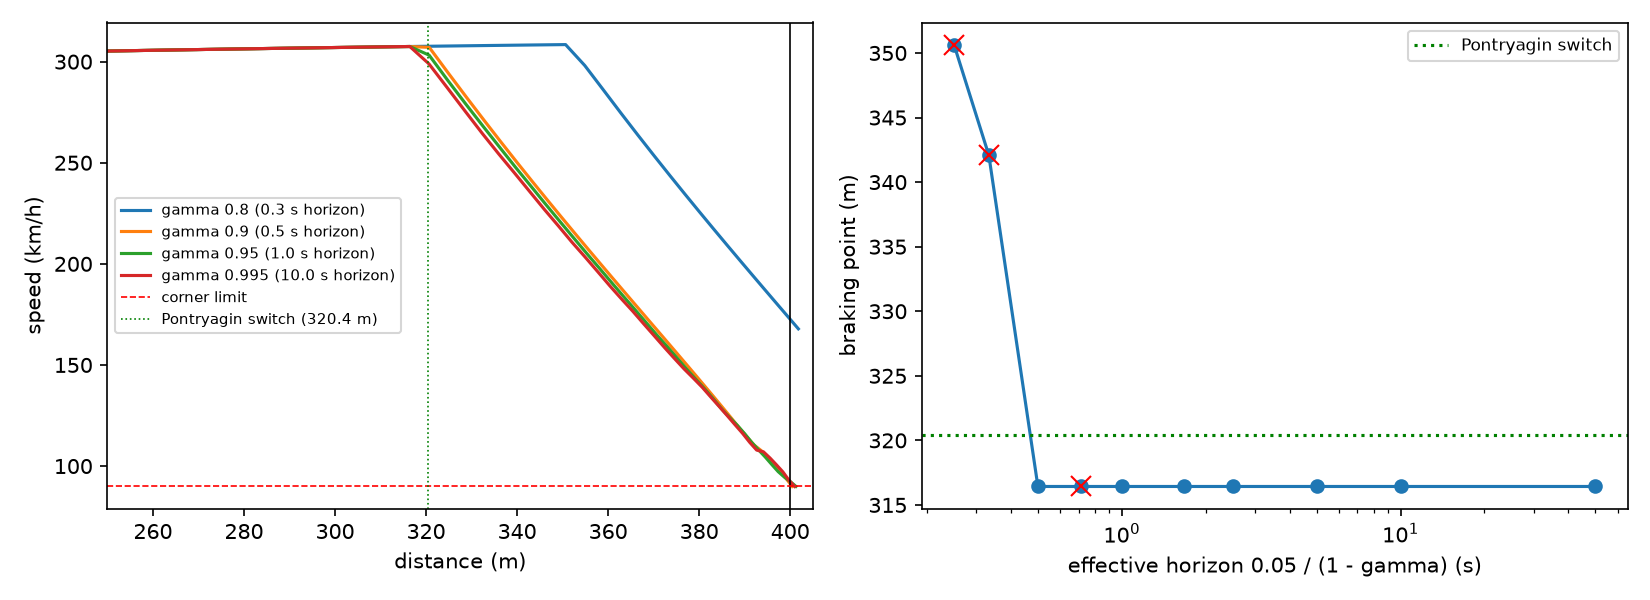
\includegraphics[width=\linewidth]{braking-gamma.png}
\caption{Left: speed against distance for four discount factors; the dotted line is
Pontryagin's switch point and the dashed line the corner's speed limit. Right: braking
point against the effective horizon; crosses mark crashes. Reproduced from the project's
findings (docs/findings/braking-gamma.png).}
\label{fig:braking}
\end{figure}

\paragraph{Reading} A crash forfeits all future progress, so its true cost is the
discounted value of everything after the corner. With a horizon of a few tenths of a
second that value is small, braking later gains more progress than the crash costs, and
the agent arrives at 144--168\,km/h. From $\gamma = 0.9$ on, every discounted optimum
brakes at 316.4\,m, one 50\,ms control step before Pontryagin's switch.
% src: docs/findings/braking-gamma.md ("Reading"); docs/STATUS.md (K3 row: "one 50 ms control
%      step before Pontryagin's switch point")

\paragraph{What this supports} Three things in the main text. First, the agent's objective
is not minimum time, and at short horizons the two optima disagree qualitatively; an
answer key built on lap time would charge such an agent with ``regret'' for doing exactly
what its objective asks. Second, at the $\gamma = 0.995$ the agent uses, the discounted and
minimum-time optima agree to within one control step on this problem, so the dense
progress reward produces racing behaviour without any lap-time term. Third, it is an
exact, independent check that a discounted optimum computed from the environment's reward
and crash penalty behaves as expected. The caveat is scale: this is a point mass in one
dimension, and the full-car counterpart is the TO-OCP itself.
